\documentclass[a4paper]{article}

\usepackage[english]{babel}
\usepackage[utf8]{inputenc}
\usepackage{amsmath}
\usepackage{graphicx}
\usepackage[colorinlistoftodos]{todonotes}
\usepackage{hyperref}
\usepackage{rotating}

\title{TOASTER, Situation Assessment Framework for Human Robot Interaction}

%\author{Grégoire Milliez, Jain Shipra}

\date{\today}

\begin{document}
\maketitle

\begin{abstract}
This document aims to explain TOASTER framework from architecture and conceptual level to implementation and computation details.
\end{abstract}

\tableofcontents

\section{Introduction}

To understand the environment, the robot needs not only to perceive it but also to reason on the relationships between the different elements and the evolution of the properties describing the world state. This understanding of its surrounding is key in order for the robot to take appropriate decisions according to the situation. TOASTER (Tracking Of Agents and Spatio-TEmporal Reasoning), is a \textbf{generic multi-sensor situation assessment framework for human-robot interaction} able to maintain a \textbf{world state}, generate \textbf{symbolic facts} from geometric computations, track \textbf{human motion} and maintain a belief state for the robot(s) as well as an estimate of the \textbf{belief state} of its human partners. The framework consists in several components, each with its specific spatial and temporal reasoning.

\subsection{Brief history}
TOASTER development started in September 2015 in LAAS-CNRS\footnote{https://www.laas.fr}.
A previous software named SPARK\footnote{https://www.openrobots.org/wiki/spark} \cite{Milliez2014}
was used in LAAS for situation assessment. TOASTER was made to replace SPARK with a modular framework.
It currently is at the version $0.4$ and the framework consists in several modules.

\subsection{Why using TOASTER?}
 
TOASTER aims to be a generic situation assessment framework, using versatile sensor inputs. It also aims to build several levels of situation assessment: from world representation to human mental state representation. TOASTER is easily extensible both on the inputs (extending supported sensors) and on the framework itself by using a modular approach. We created modules to estimate the situation of the world and of the agents. In addition, it represents and keeps track of human mental state.

TOASTER was successfully used in several applications of human robot interaction. One of the first application was to use it as a situation assessment component for an adaptive and proactive human aware robot guide \cite {fioreicsr2015}.
For this application, the robot needs to guide a group of users, through a crowded area, to bring them to a chosen location.
One of the challenges in this work was to guide people in a socially acceptable and comfortable manner. To do so, the robot had to adapt its speed to the group in order to lead everyone to the destination with a pace that satisfies most of the users and prevent user disengagement.
Another project aimed to build a robot to work with a human in an assembly line. In this scenario, the robot shares the working space with a human. Therefore, understanding the human spatial situation and current activity is key.
TOASTER, being able to provide  both low and higher level (belief state awareness) situation assessment, was used in a human robot interaction task to build the world state, monitor human actions and track human beliefs. As described in \cite{fiore2016}, the system uses agent belief awareness provided by TOASTER along with action recognition and context to enhance the robot with intention recognition capacities, which permits to give proactive behavior from the robotic system.
The semantic world representation computed by TOASTER enable to build a common ground to understand human requests and to generate appropriate speech utterances, such as "bring me the object on the kitchen's table" or even understanding when a human ask a request using multimodal language (such as pointing). In \cite{simpar_2014}, we use TOASTER along with the MORSE simulator for dialog strategy learning.

Some of our latest works aimed to model the human mental state concerning the shared plan to have an adaptive robot partner.
These works use the situation assessment frameworks like TOASTER to understand the world state but also to assess the human knowledge on the plan and update it when needed.


%TODO: show directly in which topic it can be useful and how
%Maybe just put subsection, like \subsection{situated dialogue} \subsection{Robot Guide} \subsection{intention recognition}



\section{Installation Instructions}
To install TOASTER you will need boost, ROS and toaster-lib. The ROS package Rviz is also used to visualize the data from TOASTER.

To get full instructions to install TOASTER, please refer to the wiki at
\url{https://github.com/Greg8978/toaster/wiki/installationr}.

%%%%%%%%%%%%%%%%%%%%%%%%%%%%%%%%%%%%%%%%%%%%%%%%%%%%%%%%%%%%%%%%%%%%%%55
\section{toaster-lib}
toaster-lib is a C++ library which defines data structures used in TOASTER. The structures are:
\begin{itemize}
\item \textbf{Entity}: this class defines a physical element of the world. It can be an agent or a joint or an object.

\begin{itemize}
\setlength{\itemindent}{+.0in}
\item \textbf{Agent}: this class defines an entity which has a set of joints. This agent can be a Human or a Robot.

\begin{itemize}
\item \textbf{Human}: this class represents a human agent.
\item \textbf{Robot}: this class represents a robotic agent.
\end{itemize}


\item \textbf{Joint}: this class defines an entity which belongs to an agent.
Despite its name, this can be any part of the agent's body: head, wrist, hand, gripper...
\item \textbf{Object}: this class defines an object. This object can be a MovableObjet or a StaticObject.

\begin{itemize}
\item \textbf{MovableObject}: this class defines objects that may move during the interaction.

\item \textbf{StaticObject}: this class defines objects that can't move.
\end{itemize}
\end{itemize}



\item \textbf{Area}: this class defines an area. An area is a defined location of the environment.

\begin{itemize}
\item \textbf{PolygonArea}: this class defines a polygonal area.
\item \textbf{CircleArea}: this class defines a circular area.
\end{itemize}
\end{itemize}

The attributes and links between these class are shown in the UML diagram at the figure \ref{fig:umltoasterlib}.
These key concepts (data structures) are used by TOASTER to represent the world state and to perform geometrical computations in order to obtain situation awareness for human-robot interaction. Apart from this, toaster-lib defines frequently used mathematical functions and aims to work with object-oriented approach.


%UML graph
\begin{figure}
  \centering
  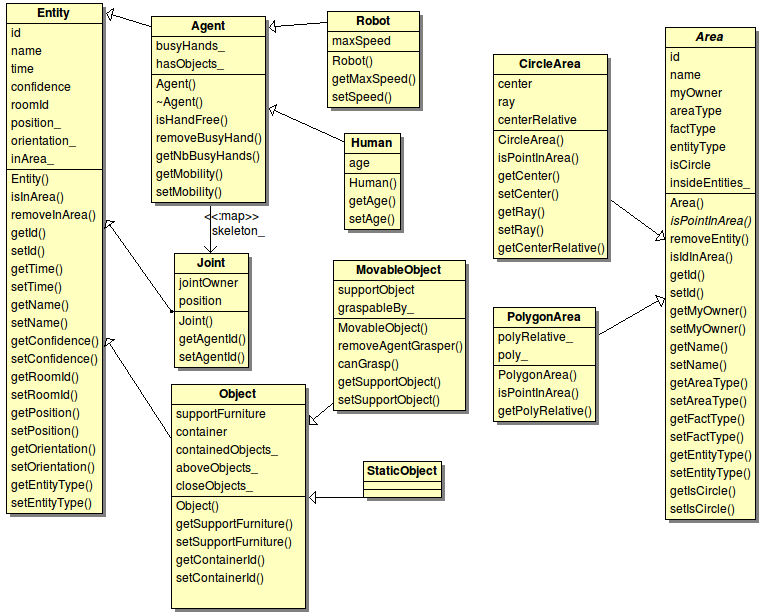
\includegraphics[width=0.99\textwidth]{img/uml_toasterLib.png}
  \caption{UML diagram from toaster-lib representing the different class and their attributes.}
  \label{fig:umltoasterlib}
\end{figure}

\section{Global Architecture}
\label{sec:architecture}
TOASTER is a modular framework. Therefore, each component can be used independently and the framework configuration can be adapted to the requirement of the chosen application.
As an example, it is possible to abstract the lower level and directly use the database by adding facts to the database tables through requests from scripts or external components.

However, some components can use data provided by other components. Fig.~\ref{fig:architecture} presents how the modules can be linked together and shows a global representation of the situation assessment architecture.

 \begin{figure}[ht!]
 \centering
 \begin{tabular}{cc}
  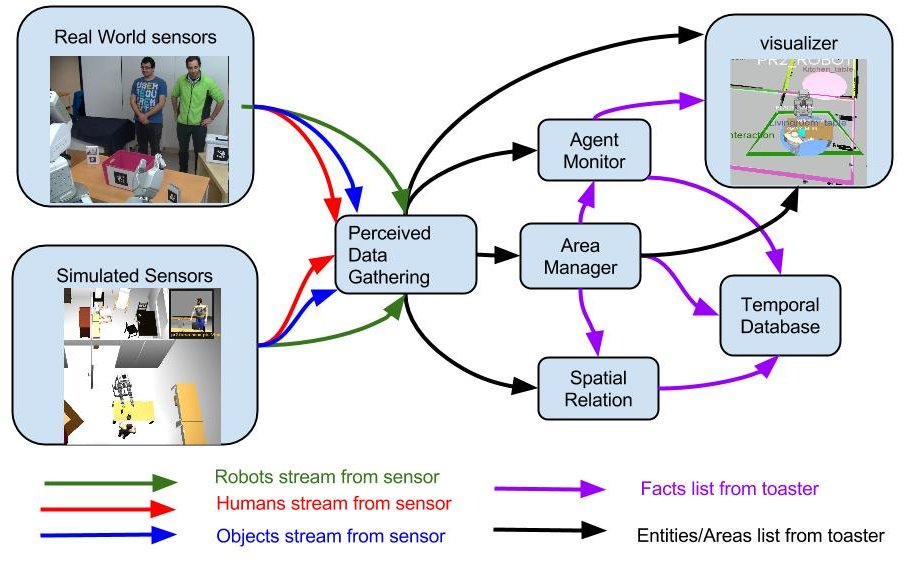
\includegraphics[width=0.9\textwidth]{img/toasterArch.jpg}
 \end{tabular}
 \caption{TOASTER architecture and interactions of the situation assessment components}
 \label{fig:architecture}
 \end{figure}


%%%%%%%%%%%%%%%%%%%%%%%%%%%%%%%%%%%%%%
\section{tools}
This repository is made to share tools linked to toaster.
One of the repositories is \textit{toaster-scripts}. It contains launch files and scripts.

It contains roslaunch files to launch several nodes of the toaster architecture with some parameters.
As an example, the roslaunch file at  \textit{roslaunch/toaster\_simu.launch} is running \textit{toaster\_simu}, \textit{pdg}, \textit{agent\_monitor}, \textit{area\_manager}, \textit{toaster\_visualizer} and \textit{rviz}. For \textit{pdg} is uses parameters defined in \textit{pdg/params/toaster\_simu.yaml} so that pdg uses topics from \textit{toaster\_simu} as input.

This repository also provides shell scripts. As an example the script \textit{/shell/spencer/area\_spencer2.sh} will send requests to \textit{area\_manager} to configure areas around a guiding robot as shown in \ref{fig:areaspencer}.

 \begin{figure}[ht!]
 \centering
 \begin{tabular}{cc}
  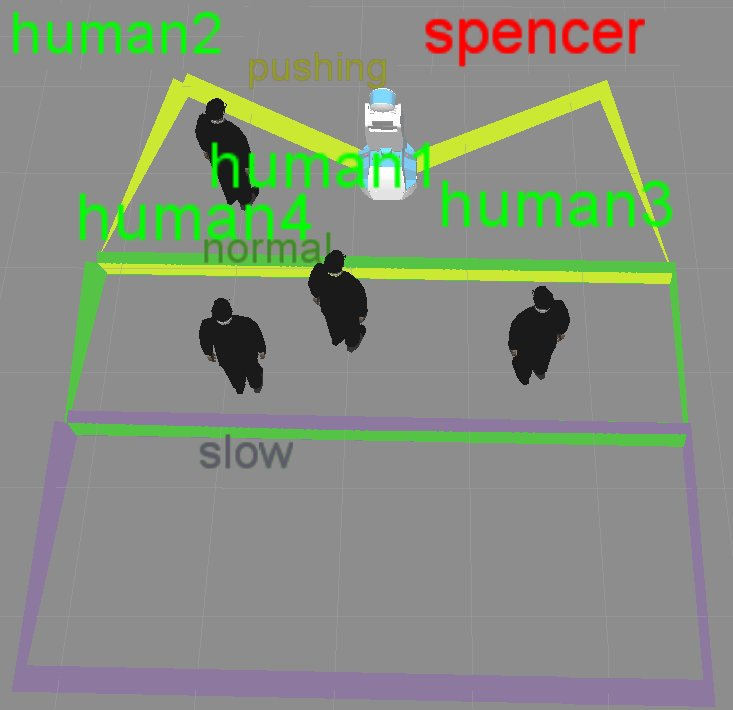
\includegraphics[width=0.9\textwidth]{img/toaster_spencer.jpg}
 \end{tabular}
 \caption{Areas are created and attached to the robot to assess the situation of the following group.}
 \label{fig:areaspencer}
 \end{figure}

In the \textit{tools} repository, we also provide python script.
As an example, the python script in \textit{python/simu\_set.py} is calling services in \textit{toaster\_simu} and \textit{agent\_monitor} to configure the environment as in \ref{fig:areaspencer} and to set an agent \textit{Greg} as a keyboard controlled entity and a monitored agent.

 \begin{figure}[ht!]
 \centering
 \begin{tabular}{cc}
  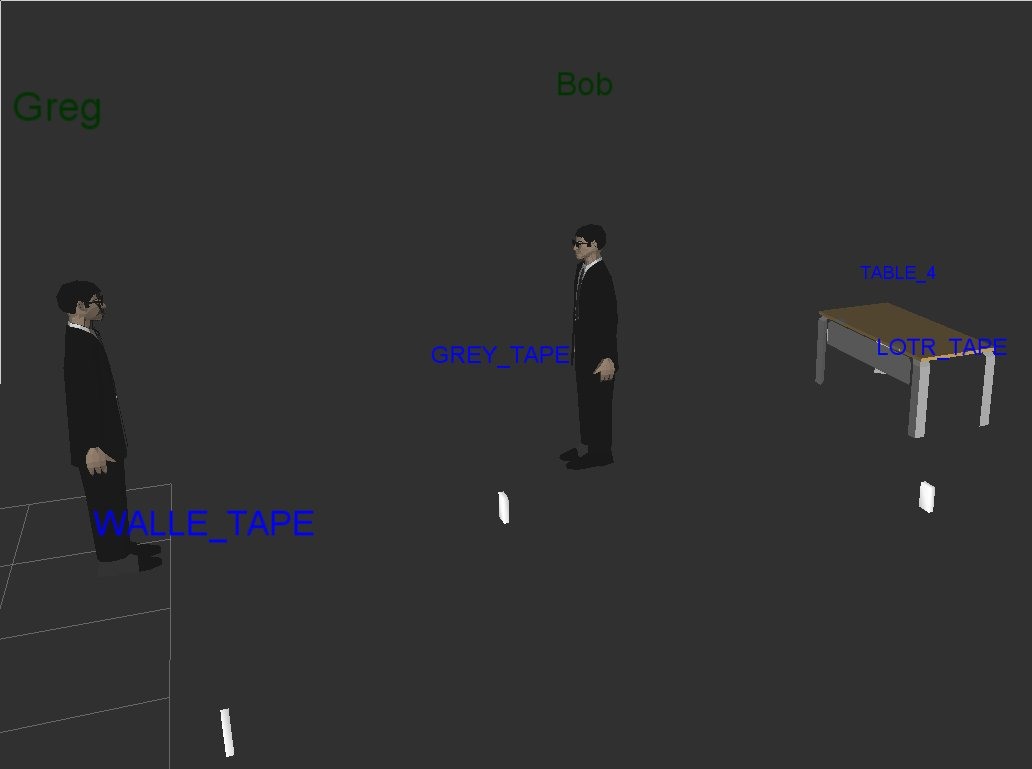
\includegraphics[width=0.9\textwidth]{img/pythonToast.jpg}
 \end{tabular}
 \caption{Environment setup from python/simu\_set.py script.}
 \label{fig:areaspencer}
 \end{figure}

%%%%%%%%%%%%%%%%%%%%%%%%%%%%%%%%%%%%%%
\section{toaster\_msgs}
This package defines all ROS messages and services used in TOASTER. All the messages type like Area, Agent, Entity, Fact, etc, have been defined in msg folder while service like AddAgent, AddArea, etc, in srv folder. Descriptions in .msg and .srv files makes it easy for ROS tools to automatically generate source code for the message type in several target languages.


\subsection{Implementation details}

toaster\_msgs includes uses one message type in defining another higher level of message. This establishes relationship of hierarchy and aggregation among various messages, can be seen in Fig.~\ref{fig:relationship}. Services used in various modules are described in subsequent sections. To see the detailed structure of each messages refer to \url{https://github.com/Greg8978/toaster/tree/master/toaster_msgs/msg} and for services: \url{https://github.com/Greg8978/toaster/tree/master/toaster_msgs/srv}.

This package also provides classes to help other modules to read the messages and to convert then into \textit{toaster-lib} data structure.
These class are \textit{ToasterFactReader, ToasterObjectReader, ToasterHumanReader, ToasterRobotReader}. 
% relationship between messages

 \begin{figure}[ht!]
 \centering
 \begin{tabular}{cc}
  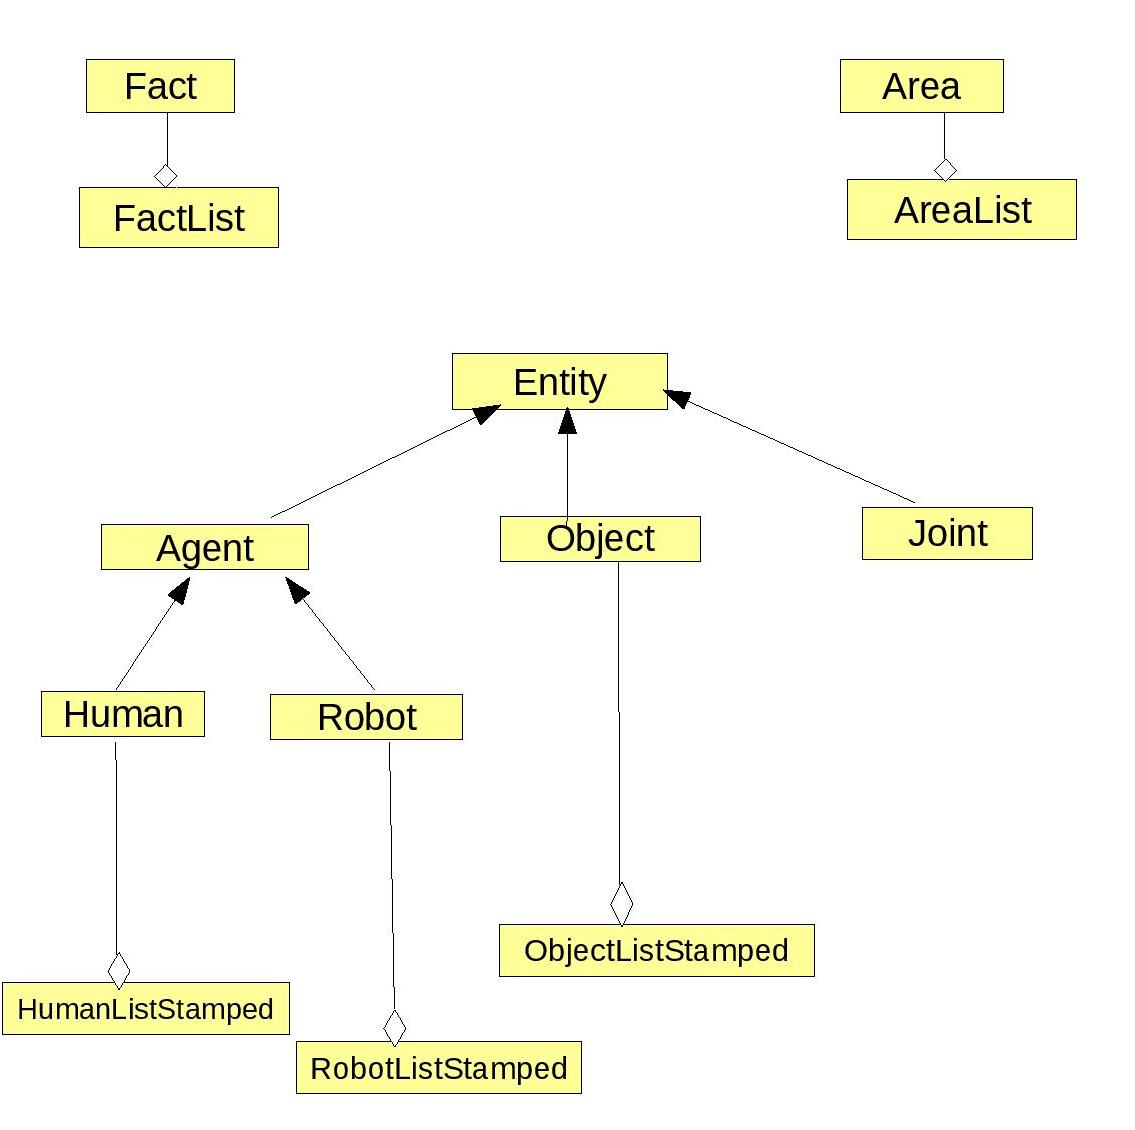
\includegraphics[width=0.90\textwidth]{img/msgRelationship.jpg}
 \end{tabular}
 \caption{Relationship between .msg structures in toaster\_msgs}
 \label{fig:relationship}
 \end{figure}
 
 
\subsection{Symbolic representation and fact}
Our situation assessment modules perform geometric computations to get a symbolic representation of the world. This symbolic representation is made based on a list of a data structure named a \textit{fact}. In our system, a \textit{fact} is a vector, with several fields, used to represent a property of the environment. We detail below the fields of this vector.
\begin{itemize}
\item \textit{Subject}: the entity on which the property applies (e.g.: \textit{Red\_Mug}, \textit{Human1}, \textit{Pr2}, \textit{Human\_Right\_Hand}).
\item \textit{Property}: the property linked to the \textit{Subject} (e.g.: \textit{isOn}, \textit{isFull}, \textit{isMoving}, \textit{isPointing}, \textit{canSee}).
\item \textit{Target}: the property may link the entity-subject with an entity-target. As an example if an entity \textit{BOOK} is on an entity \textit{TABLE}, \textit{BOOK} will be the subject while \textit{TABLE} will be the target.
\item \textit{PropertyType}: this parameter defines the category in which the property falls (e.g.: \textit{position}, \textit{state}, \textit{motion}, \textit{posture}, \textit{affordance}). Using this parameter, if an external module adds a fact, it is still possible to know which kind of property it is.
\item \textit{Value}: a property may have a value linked to it. As an example, the property \textit{isFull} or \textit{isMoving} may have the value \textit{TRUE} or \textit{FALSE} (if we want to have a close world representation). As another example, if we represent the distance between joints, such as robot's hand to human head, the \textit{Value} parameter could be set to \textit{DANGER}, \textit{CLOSE} or \textit{FAR}, or even holds a numerical value.
In some situations, to represent a lack of knowledge on a property and the awareness of this lack, the fact's value can also be set to \textit{unknown}.
\item \textit{Confidence}: this figure between 0 and 1 represents the reliability of the fact. This can be linked to sensor reliability or to the property computation itself.
\item \textit{Time}: the time at which the fact was computed.
\item \textit{FactObservability}: the probability that a human would acquire the awareness of the fact if he sees the Subject of the fact. 
\end{itemize}

As an example, the vector
%TODO Make this as a table?
$<$ $Subject = Bob\_Right\_Hand$, $Property = isMovingToward$, $Target = Red\_Book$, $PropertyType = motion$, $Confidence = 0.8$, $time = 145571646570$, $FactObservability = 0.7$ $>$ represents the fact that, at the given time, the hand (\textit{Bob\_Right\_Hand}) of Bob is going toward a book (\textit{$Red\_Book$}) with a confidence of \textit{0.8}. 
The following sections describe spatial and temporal reasoning components that generate these kind of facts.

%\subsection{Future work and possible improvement}







%%%%%%%%%%%%%%%%%%%%%%%%%%%%%%%%%%%%%%
\section{toaster\_simu}

\textit{toaster\_simu} is an inbuilt-simulation component of TOASTER which allows to add entities (objects, robots, humans and joints)
and provides the desired environment to TOASTER for situation assessment.
This makes possible to quickly set up an interaction environment in order to test new features or new modules without requiring any robotic device or any real environment.


\subsection{Implementation details}
Fig.~\ref{fig:toastersimu} gives an idea of the implementation of services and topics in toaster\_simu.

% block diagram for toaster_simu

 \begin{figure}[ht!]
 \centering
 \begin{tabular}{cc}
  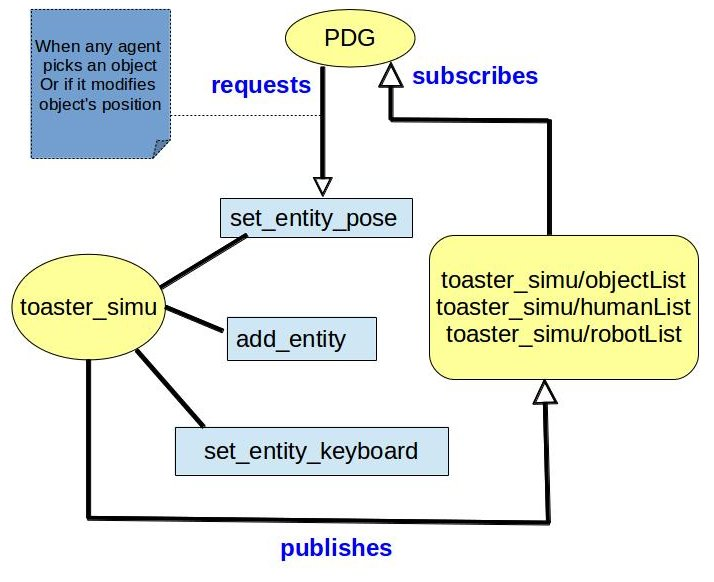
\includegraphics[width=0.9\textwidth]{img/toasterSimu.jpg}
 \end{tabular}
 \caption{toaster\_simu services and messages. Ellipses represent nodes, rectangles represent services and messages.}
 \label{fig:toastersimu}
 \end{figure}



\subsection{Inputs}
Inputs for this module are id, type and position of entities to be added to the environment being assessed. They are provided through services as described below. Another set of inputs will be from keyboard if any entity is teleoperated (see fig.~\ref{fig:directions} for keyboard teleoperation keys).

\begin{figure}[ht!]
 \centering
 \begin{tabular}{cc}
  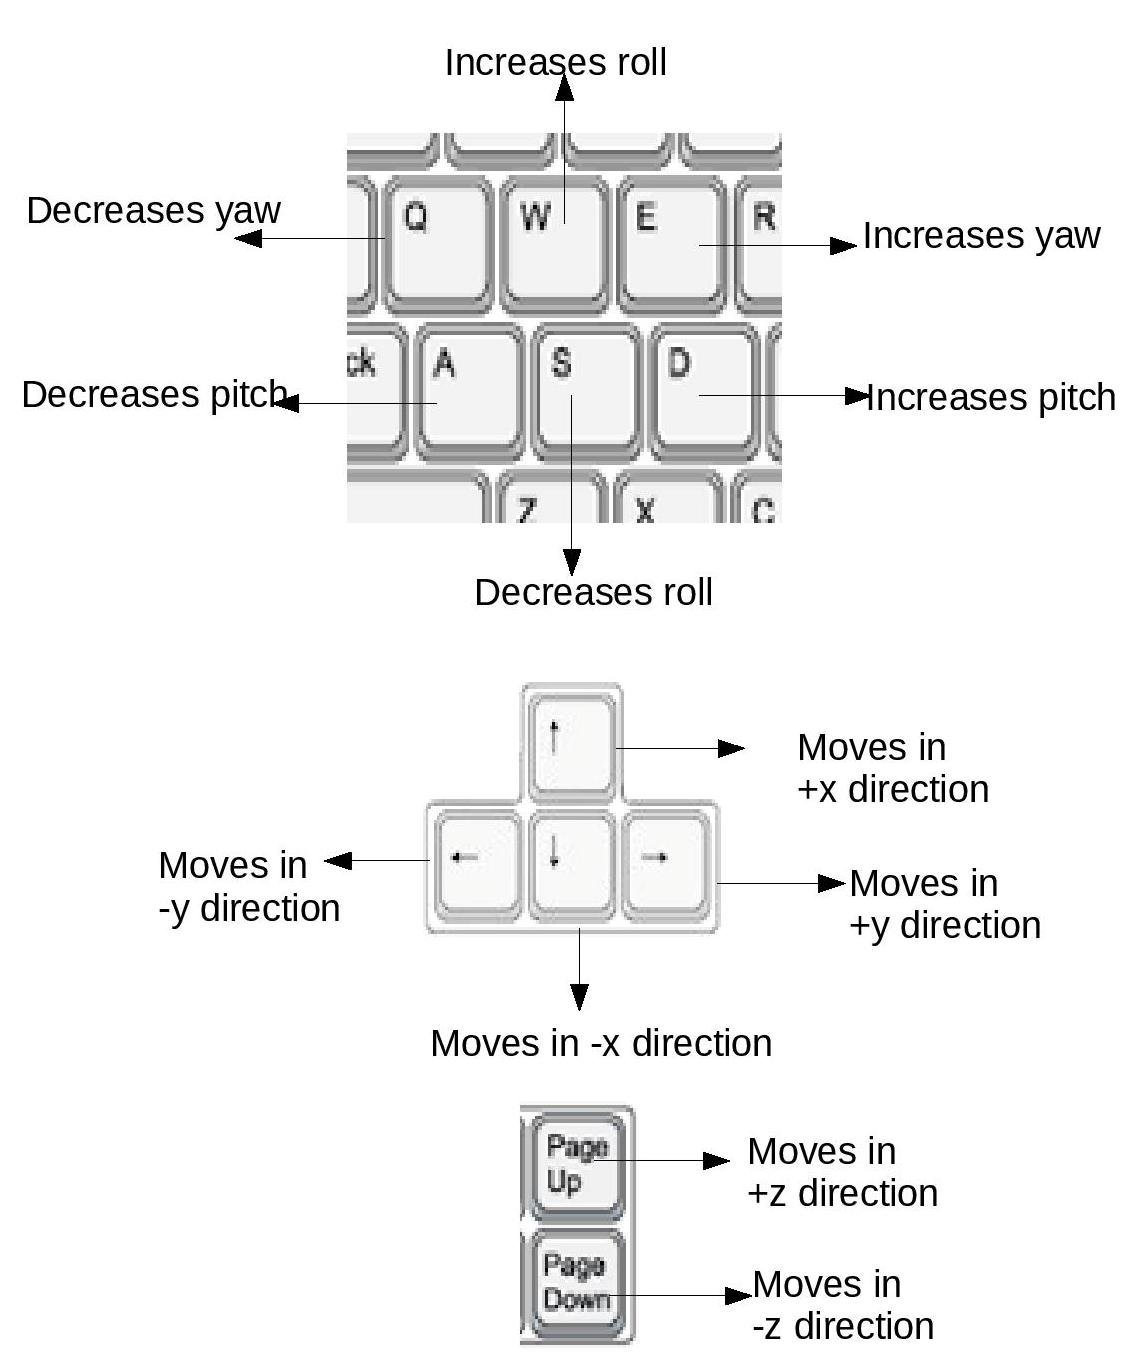
\includegraphics[width=0.9\textwidth]{img/directions.jpg}
 \end{tabular}
 \caption{keys to control the entity}
 \label{fig:directions}
 \end{figure}

\subsection{Outputs}
Outputs for toaster\_simu component are published on topics \textit{/toaster\_simu/humanList}, \textit{/toaster\_simu/robotList} and \textit{/toaster\_simu/objectList} which are subscribed by higher level component PDG.

\subsection{Services}
This component provides the following services :

\begin{itemize}
\item \textbf{add\_entity} - enables you to add an entity to the environment. It takes a string \textit{id} to give to the entity, a string \textit{name} which will be also use to find the corresponding 3D model, a string \textit{type} which should be set to the entity type (human, robot, object or joint). The last parameter is the string \textit{ownerId}. It is used for joint entities to give the id of the agent it belongs to.

\textbf{Shell command to call the service:}
\textit{rosservice call /toaster\_simu/add\_entity "id: ''
name: ''
type: ''
ownerId: ''"}


\item \textbf{remove\_entity} - enables you to remove an entity from the environment. It takes strings to identify the entity.

\textbf{Shell command:}
\textit{rosservice call /toaster\_simu/remove\_entity "id: ''
type: ''
ownerId: ''"}

\item \textbf{set\_entity\_keyboard} - enables you to set any entity to keyboard mode so that it can be controlled by keyboard. It takes a sting with the id of the entity you want to control.

\textbf{Shell command:}
\textit{rosservice call /toaster\_simu/set\_entity\_keyboard "id: ''"}

\item \textbf{set\_entity\_pose:} - enables you to set position of any existing entity. The three first parameters \textit{id, ownerId, type} are strings meant to identify the entity whose position is to be changed. The last parameter is the pose in which we want to put the entity with the type \textit{geometry\_msgs/Pose} from ros.

\textbf{Shell command:}

\textit{ rosservice call /toaster\_simu/set\_entity\_pose "{id: '', 
 ownerId: '', 
 type: '', 
 pose:
  position:
    x: 0.0
    y: 0.0
    z: 0.0
  orientation:
    x: 0.0
    y: 0.0
    z: 0.0
    w: 0.0"}" }
 
 
\end{itemize}


\subsection{Limitations and improvements}
The current version of toaster\_simu allows to quickly add or remove any kind of entity from the environment. However, as it is meant to be a tool for quick testing, it doesn't provide a simulation of perception as a simulator would do but directly add a "perceived" world state. Nevertheless, TOASTER  is also compatible with inputs from the robotic open-source software MORSE.

An other limitation is that an agent can be added with his joints, however for now, the joint position is not updated with the agent's one\footnote{see \url{https://github.com/Greg8978/toaster/issues/19}}.


%%%%%%%%%%%%%%%%%%%%%%%%%%%%%%%%%%%%%%
\section{Perceived Data Gathering}
In a scenario of human-robot interaction, data concerning three entities (humans, objects and robots) may come from various sensors with heterogeneous data-types. As we wish to keep the geometrical reasoning generic while having a flexible data-source system, we use a separate component PDG (Perceived Data Gathering) to collect the data from all the required sensors and publish them in a unique format usable by any other TOASTER component.






\subsection{Implementation details}
The current version already supports several inputs. For human tracking, TOASTER can get data from kinect-like and motion capture devices. Concerning objects, an object recognizer based on tags and stereo vision is supported. Finally, two different models of robots are directly functional in TOASTER. However the set of inputs is easily extensible by adding a new sensor data reader to the \textit{PDG} module. Additionally, TOASTER can use HRI simulators. The robotic simulator MORSE\cite{simpar_2014} \cite{lemaignan2014simulation} and a built-in simulation component (toaster\_simu) are supported as inputs for any type of entities (objects, humans or robots). These two simulators allow to quickly test TOASTER components and allow to have a partially simulated interaction. As an example, we can have a real human interacting with a simulated robot by using data obtained from a motion capture for the human in real world, and data from a simulator output for the robot pose. The figure \ref{fig:pdg} illustrates the messages and services provided by \textit{PDG}

 \begin{figure}[ht!]
 \centering
 \begin{tabular}{cc}
  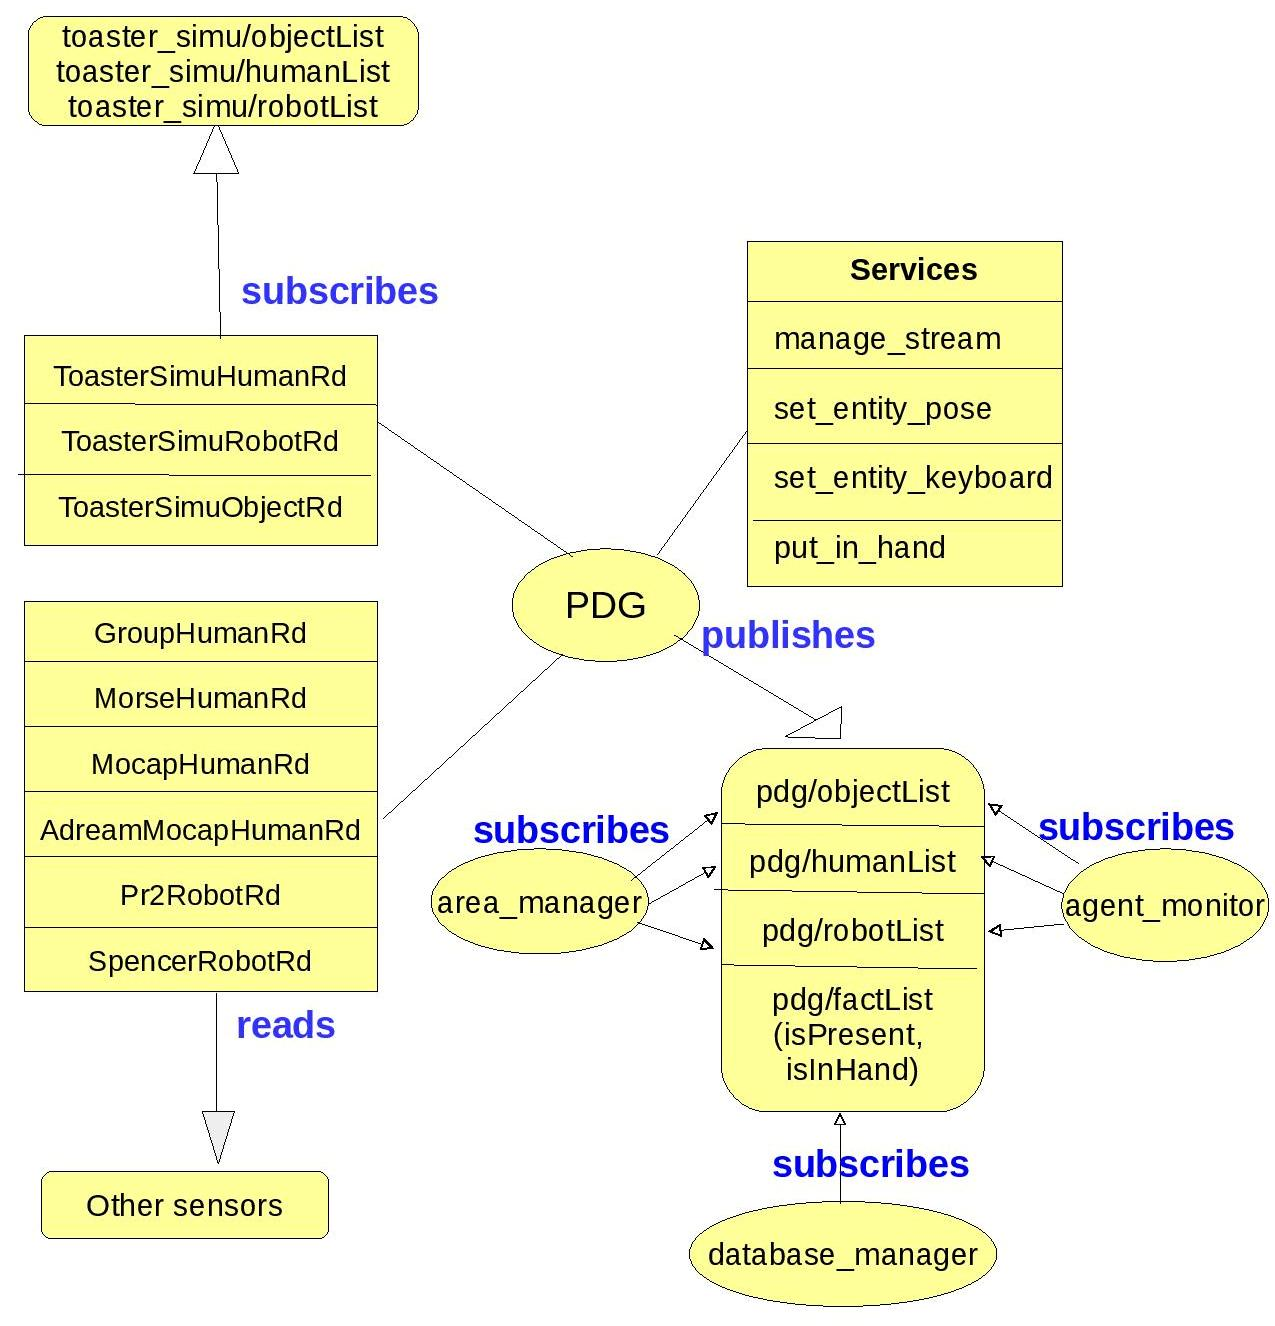
\includegraphics[width=0.90\textwidth]{img/pdg.jpg}
 \end{tabular}
 \caption{Implementation details of Perceived Data Gathering module}
 \label{fig:pdg}
 \end{figure}
 
 
 \subsection{Facts computation}
%TODO: list of computed facts and how are they computed?

The facts generated by this module are:

\begin{itemize}
\item \textbf{IsInHand}: this fact is produced when an object has been set in an agent's  hand. The \textit{property} is \textit{IsInHand}, the \textit{propertyType} is \textit{position}, the \textit{subProperty} is \textit{object}, the \textit{subjectId} is the id of the object, the \textit{targetId} is the id of the joint (hand), the \textit{targetOwnerId} is the id of the agent, the \textit{time} is set with the perception time of the joint, the \textit{valueType} is set to zero and the \textit{stringValue} is set to \textit{true}.
\item \textbf{IsSeen}: this fact is produced to tell that an object is currently seen (detected) by the robot. The fact \textit{property} is \textit{IsSeen}, the \textit{propertyType} is \textit{affordance}, the \textit{subjectId} is the id of the object perceived. The \textit{time} of the fact is set using the time of the object perception. The \textit{valueType} is set to zero and the \textit{stringValue} is set to \textit{true}. 

\end{itemize}
 
\subsection{Inputs}
The data streams about position, orientation and other properties of humans, robots, objects and joints from various sensors like kinect act as an input for this module.
\subsection{Outputs}
%TODO: give the name of the topics here and what is inside
Output is the sensor data published on various topics with well-defined data structure.
\subsection{Services}
On running this node, one can access following services:
\begin{itemize}
\item \textbf{manage\_stream} - It enables to specify, at any moment, which sensor's data to use as raw input by putting the corresponding flag at \textit{true}. This makes the PDG component highly adaptable to the data needed for the current task and to the set of available sensors. 

\textbf{Shell command:}
\textit{rosservice call /pdg/manage\_stream "{morseHuman: false, niutHuman: false, groupHuman: false, mocapHuman: false, adreamMocapHuman: false,
  toasterSimuHuman: false, pr2Robot: false, spencerRobot: false, toasterSimuRobot: false,
  toasterSimuObject: false}}
  
\item \textbf{set\_entity\_pose} - enables you to set position of any existing entity. The three first parameters \textit{id, ownerId, type} are strings meant to identify the entity whose position is to be changed. The last parameter is the pose in which we want to put the entity with the type \textit{geometry\_msgs/Pose} from ros.

\textbf{Shell command:}

\textit{ rosservice call /toaster\_simu/set\_entity\_pose "{id: '', 
 ownerId: '', 
 type: '', 
 pose:
  position:
    x: 0.0
    y: 0.0
    z: 0.0
  orientation:
    x: 0.0
    y: 0.0
    z: 0.0
    w: 0.0"}" }
 

\item \textbf{put\_in\_hand} - This service has provision of adding an object in any agent's hand. It actually links the object position to a joint. All three inputs are of string type to define the object and the joint.

\textbf{Shell command:}
\textit{rosservice call /pdg/put\_in\_hand "objectId: ''
agentId: ''
jointName: ''" }

\item \textbf{remove\_from\_hand} - It enables to remove object from agent's hand. It takes a string \textit{objectId} of the object that is to be removed.

\textbf{Shell command:}
\textit{rosservice call /pdg/remove\_from\_hand "objectId: ''" }

\end{itemize}
%\subsection{Examples}


\subsection{Limitations and possible improvement}
\textit{PDG} is meant to aggregate data from various sensors.
It is possible to use several modalities to get the same entity's position.
For now, there is no way to manage a conflict if several sensors detect the same object with a different position.

An other way to improve \textit{PDG} is to add supported inputs. This can be easily done by using heritage from one of the class \textit{ObjectReader, RobotReader} or \textit{HumanReader} according to what kind of entity is localized by the sensor.



%%%%%%%%%%%%%%%%%%%%%%%%%%%%%%%%%%%%%%
\section{area\_manager}
We define an area as a bounded region in the environment with semantic meaning. This module associates area with the entity to calculate their interaction with other entities. These areas are useful to get a first discrimination of the situation and conditional computation.

\subsection{Implementation details}
In the current implementation, an area is bi-dimensional (however the concept is still valid for tri-dimensional areas). Areas can be a polygon or a circle, static or dynamic. In TOASTER, areas have several parameters: \textit{areaType, factType, entityType, owner}. The \textit{areaType} defines the category of the area (such as room, escalator, television\_area). As areas could be used for different situation, we use the \textit{factType} to define what type of calculation needs to be done for entities inside the current area. This parameter is very linked to the semantic of the area. The \textit{entityType} defines what kinds of entities are concerned by the area. Entities which are not in the category will be ignored. Finally, \textit{owner} defines which entity "owns" this area. If set, the area is updated with the owner's position and orientation. For a clear relationship between pdg node with its topics, services and other nodes, refer Fig.~\ref{fig:areaManager}.

 \begin{figure}[ht!]
 \centering
 \begin{tabular}{cc}
  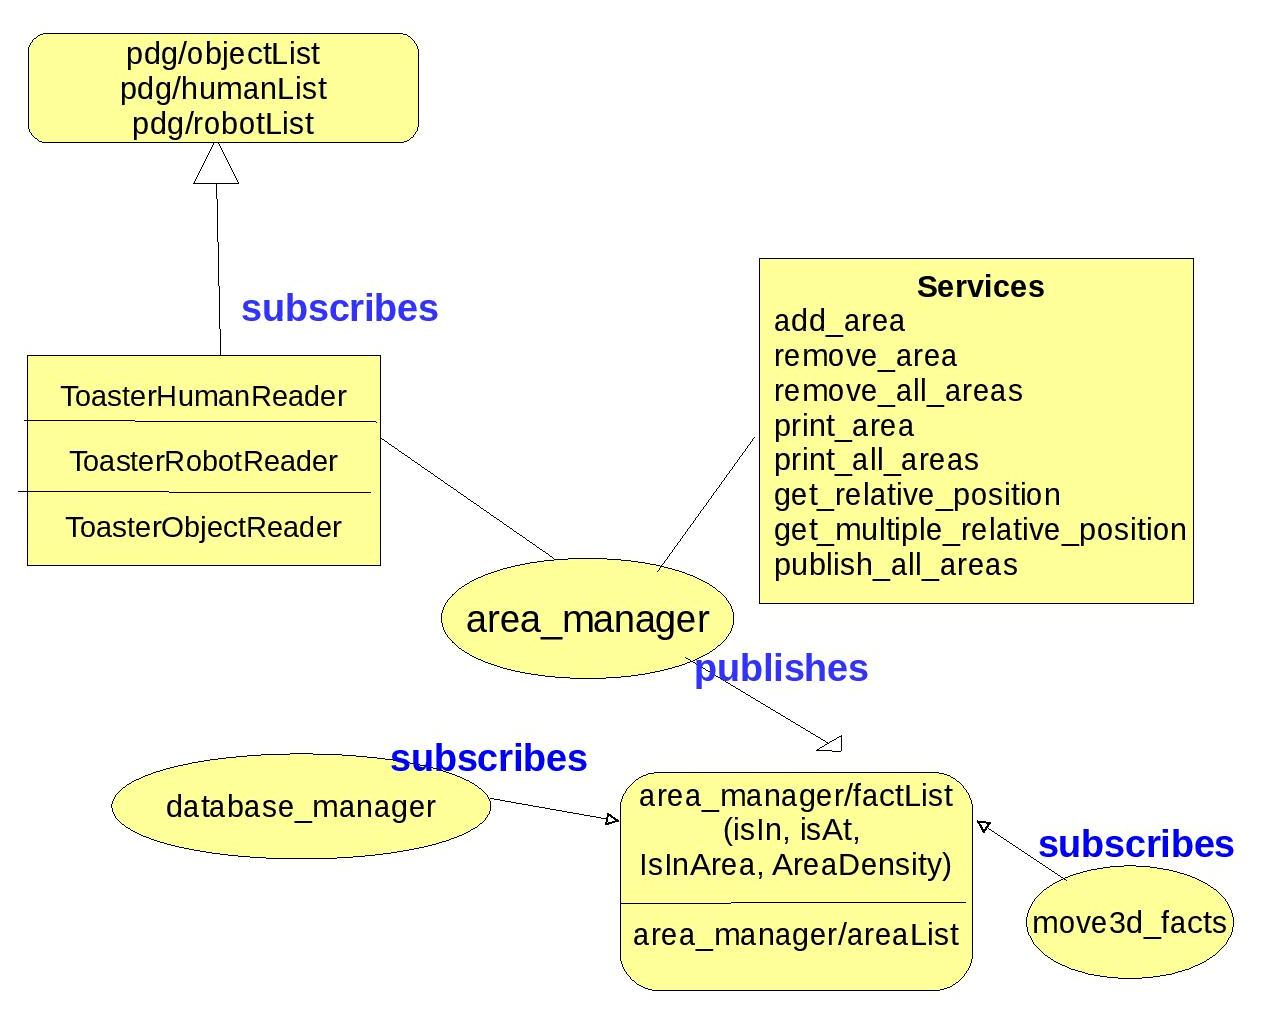
\includegraphics[width=0.90\textwidth]{img/areaManager.jpg}
 \end{tabular}
 \caption{Implementation of area\_manager module}
 \label{fig:areaManager}
 \end{figure}



\subsection{Facts computation}
%TODO: list of computed facts. Replace what is there

The facts generated by this module are:

\begin{itemize}
\item \textbf{IsInRoom}: this fact is produced for area with \textit{areaType} equal to \textit{room}. When a concerned entity (an entity which belongs to the class \textit{entityType} of the room), is inside the area, this fact is generated. The \textit{property} is \textit{IsInRoom}, the \textit{propertyType} is \textit{position}, the \textit{subProperty} is \textit{room}, the \textit{subjectId} is the id of the entity inside the room, the \textit{targetId} is the name of the area, the \textit{time} is set with the perception time of the entity, the \textit{valueType} is set to zero and the \textit{stringValue} is set to \textit{true}.
\textbf{example:} \textit{Bob IsInRoom Livingroom ...}

\item \textbf{IsAt}: this fact is produced for area with \textit{areaType} equal to \textit{support}. When a concerned entity (an entity which belongs to the class \textit{entityType} of the area), is inside the area, this fact is generated. The \textit{property} is \textit{IsAt}, the \textit{propertyType} is \textit{position}, the \textit{subProperty} is \textit{location}, the \textit{subjectId} is the id of the entity inside the room, the \textit{targetId} is the name of the area, the \textit{time} is set with the perception time of the entity, the \textit{valueType} is set to zero and the \textit{stringValue} is set to \textit{true}.
\textbf{example:} \textit{Bob IsAt Livingroom\_table ...}

\item \textbf{IsInArea}: this fact is produced for any other kind of area with \textit{areaType} different to \textit{support} and \textit{room}. When a concerned entity (an entity which belongs to the class \textit{entityType} of the area), is inside the area, this fact is generated. The \textit{property} is \textit{IsInArea}, the \textit{propertyType} is \textit{position}, the \textit{subProperty} is set with \textit{areaType}, the \textit{subjectId} is the id of the entity inside the room, the \textit{targetId} is the name of the area. If the area has an \textit{owner}, we set \textit{targetOwnerId} with its id. The \textit{time} is set with the perception time of the entity, the \textit{valueType} is set to zero and the \textit{stringValue} is set to \textit{true}.
\textbf{example:} \textit{Bob IsInArea corridor ...}

\item \textbf{AreaDensity}: this fact is produced to get the density of element in an area if area has factType set to \textit{density}. The fact \textit{property} is \textit{AreaDensity}, the \textit{propertyType} is \textit{density}, the \textit{subProperty} is set with \textit{ratio}. The \textit{subjectId} is the name of the area. The \textit{time} of the fact is set using the time of the entity in the area. The \textit{valueType} is set to one and the \textit{doubleValue} is the ratio \textit{nbEntInArea}/\texttt{nbEnt}, with nbEntInArea the number of concerned entities (from the \textit{entityType} of the area) and nbEnt the total number of these entities.

\item \textbf{IsFacing}: this fact is computed for entity inside an area with \textit{interaction} as factType. We compute the orientation of the entity and we compare it with the position of the area owner. If this orientation is close enough, we consider that the entity is facing the area owner. 

The fact \textit{property} is \textit{IsFacing}, the \textit{propertyType} is \textit{posture}, the \textit{subProperty} is set with \textit{angle}. The \textit{subjectId} is the id of the entity. The \textit{targetId} is set with the id of the area's owner. The \textit{time} of the fact is set using the time of the entity perception. The \textit{valueType} is set to zero, the \textit{stringValue} is \textit{true} and the \textit{doubleValue} is the angle of deviation between the orientation toward the area's owner and the actual entity orientation.

\end{itemize}

To compute the presence of an element in an area, we use the distance from the center for circular area which we compare to the ray of the area.
For polygonal areas, we use the boost library and the \textit{within} function of the polygon (see \url{http://www.boost.org/doc/libs/1_61_0/libs/geometry/doc/html/geometry/reference/algorithms/within/within_2.html}) .


\subsection{Inputs}
area\_manager takes outputs of PDG module i.e. orientation, positions and other properties of entities. 
\subsection{Outputs}
It publishes facts like isInArea, isAt, AreaDensity on topic named \textit{/area\_manager/factList} and areas on topic \textit{/area\_manager/areaList}.

\subsection{Services}
Services provided by area\_manager are :
\begin{itemize}
\item \textbf{add\_area}- In the current implementation, an area is bi-dimensional (however the concept is still valid for tri-dimensional areas). Areas can be a polygon or a circle, static or dynamic. In TOASTER, areas have several parameters: \textit{areaType, factType, entityType, owner}. The \textit{areaType} defines the category of the area (such as room, escalator, television\_area). As areas could be used for different situation, we use the \textit{factType} to define what type of calculation needs to be done for entities inside the current area. This parameter is very linked to the semantic of the area. The \textit{entityType} defines what kinds of entities are concerned by the area. Entities which are not in the category will be ignored. Finally, \textit{owner} defines which entity "owns" this area. If set, the area is updated with the owner's position and orientation. Concerning the id of the area, if an id is given, the area will have this id, replacing the previous area with the same id if any. When no \textit{id} is specified (the default value 0 is given) the module will assign the area with the first available unsigned integer. The message format of the service looks like this:

\textbf{Shell command:}

\textit{rosservice call /area\_manager/add\_area "myArea:
  id: 0
  name: ''
  myOwner: ''
  areaType: ''
  factType: ''
  entityType: ''
  isCircle: false
  center: {x: 0.0, y: 0.0, z: 0.0}
  ray: 0.0
  poly:
    points:
    - {x: 0.0, y: 0.0, z: 0.0}
  insideEntities: [0]" }
  
\item \textbf{remove\_area} - Areas can be added and removed as per the requirements. This service is used to remove the area where input is the area's numeric id. This id is positive.

\textbf{Shell command:}

\textit{rosservice call /area\_manager/remove\_area "id: 0"}


\item \textbf{remove\_all\_area }- as the name suggests, service remove\_all\_areas removes all areas created for the situation assessment.

\item \textbf{print\_area} - This service take id of area and prints its details including its position, orientation, owner and list of entities inside this area. Similarly, the service print\_all\_areas prints details of all areas.

\item \textbf{get\_relative\_position} - This service computes relative position of target with respect to subject and shows it in higher level terms like right, left, ahead, back etc, which are simple for human understanding. It takes string id of subject and target entity.

\textbf{Shell command:}

\textit{rosservice call /area\_manager/get\_relative\_position "subjectId: ''
targetId: ''" }

\item \textbf{get\_multiple\_relative\_position} - this service is used to get relative position of an object compared to an other from an agent point of view. It takes a string \textit{agentSubjectId} of the agent from which we want the point of view, the string \textit{objectSubjectId} giving the id of the object which we will use to describe the position of the object identified by the string \textit{objectTargetId}.

\textbf{Shell command:}

\textit{rosservice call /area\_manager/get\_multiple\_relative\_position "agentSubjectId: ''
objectSubjectId: ''
targetId: ''"}

\item \textbf{publish\_all\_areas }- This service controls the publishing of areas on /area\_manager/areaList topic. If this service is called, a parameter name publishingArea\_ is negated. The node only publishes on areaList topic if this parameter is positive. By default, it is set to true.
\end{itemize}

\subsection{Examples}
As an example, it is possible to define a polygon in front of the robot (\textit{myRobot}) to know if a human is in an interaction configuration. This area triggers some computation such as the human body orientation. It would have as set of parameters <\textit{interaction, orientation, humans, myRobot}> and is updated with the position and orientation of \textit{myRobot}. This example is illustrated by the pink area of Fig.~\ref{fig:interactionarea}.

 \begin{figure}[ht!]
 \centering
 \begin{tabular}{cc}
  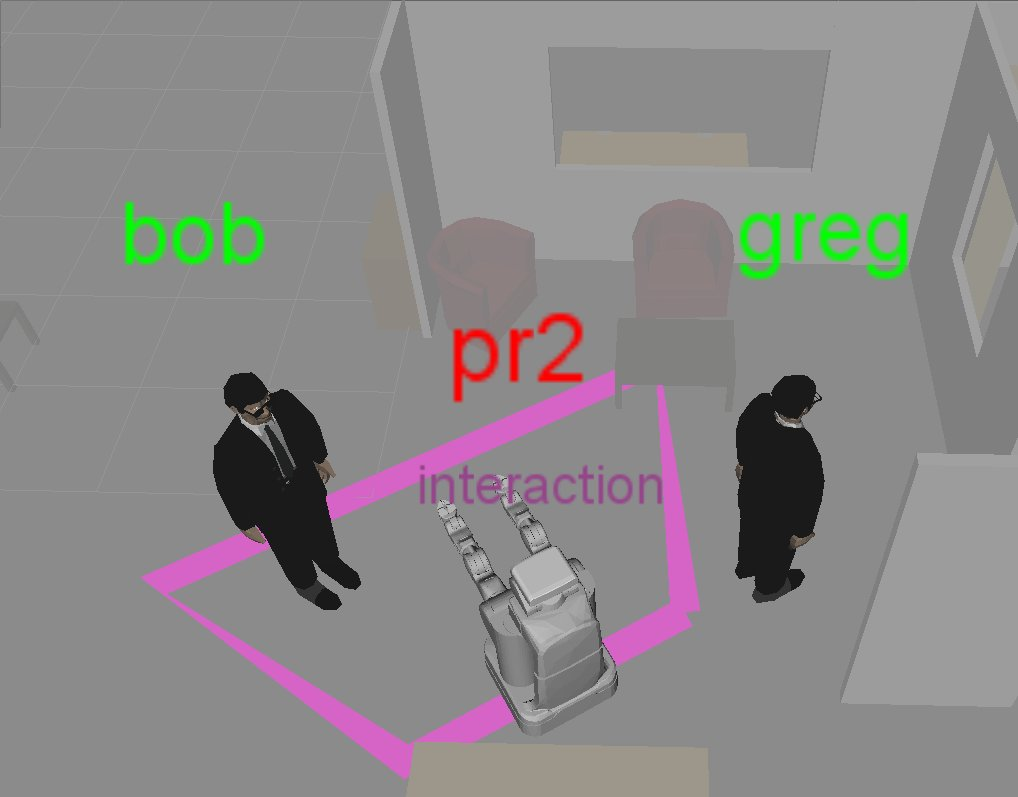
\includegraphics[width=0.90\textwidth]{img/interactionarea.jpg}
 \end{tabular}
 \caption{Illustration of an area to detect a user in "interaction" configuration (inside robot's interacting area and facing the robot).}
 \label{fig:interactionarea}
 \end{figure}

\subsection{Future work and possible improvement}
To improve this module, we should add 3d areas.
Also currently the number of areaType is quite limited. A way to improve would be to have a configuration file where we could define a new type of area and tell which facts computation should be triggered for this kind of area.
As an example, the computation of facts in \textit{move3d\_facts} or \textit{agent\_monitor} should be triggered according to the configuration with areas. As an example, it could be useless to compute if an agent isMovingToward an object when the object is not in the same room.

%%%%%%%%%%%%%%%%%%%%%%%%%%%%%%%%%%%%%%
\section{agent\_monitor}

When the robot has to perform a task collaboratively with a human partner, it is key for the robotic system to understand the human's activity. To do so, one component of the TOASTER framework, called Agent Monitoring, is computing facts concerning the agent's motion, posture and distance regarding points of interest.

\subsection{Implementation details}
To implement the desired functionality for this module, circular buffer data structure has been used. At all time, the module records the position of any entity, for a short period of time, in a time stamped circular buffer. This allow to access the entity position at a given time (supposed not too far in the past).

 \begin{figure}[ht!]
 \centering
 \begin{tabular}{cc}
  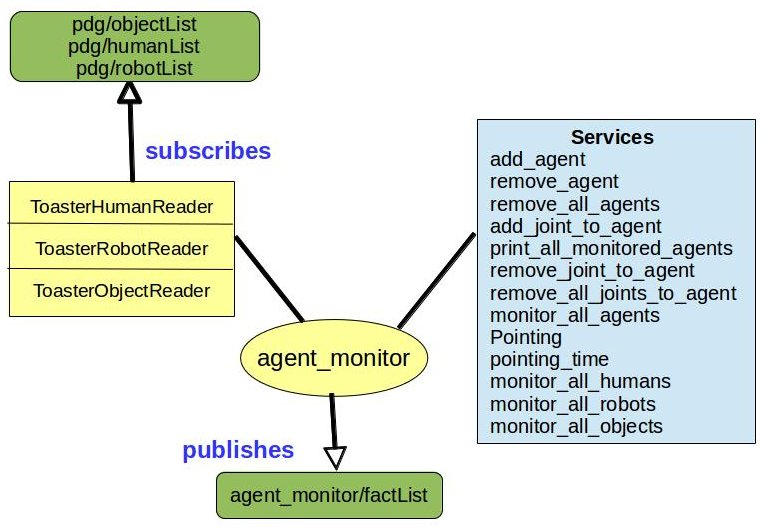
\includegraphics[width=0.90\textwidth]{img/agentMonitor.jpg}
 \end{tabular}
 \caption{Implementation of agent\_monitor
 module}
 \label{fig:agentMonitor}
 \end{figure}
 
 
\subsection{Facts computation}
%TODO: list of computed facts and how are they computed?

The facts generated by this module concerning the monitored agent's body are:

\begin{itemize}
\item \textbf{IsLookingToward}: this fact is computed for any agent monitored. It uses the head joint of the agent and an angular aperture value to compute a cone from the agent's head. If an object is in the cone, or if the "head" of an agent is in the cone, it's considered as looked.

The fact will have \textit{IsLookingToward} as \textit{property}, the \textit{propertyType} is \textit{attention}, the \textit{subProperty} is \textit{agent}, the \textit{subjectId} is the id of the monitored agent, the \textit{targetId} is the id of the entity looked upon, the \textit{time} is set with the perception time of the monitored agent, the \textit{valueType} is set to one and the \textit{doubleValue} is set with the angular distance from the center axis of the cone to the taget entity. The \textit{confidence} is set with a normalization from this angle \textit{angleEnt} to the global cone angle \textit{angleCone} : $angleCone-anlgeEnt/angleCone$.

\textbf{example:} \textit{Bob IsLookingToward LOTR\_BOOK ...}

\item \textbf{IsMoving}: this fact is produced if the monitored agent global body is in motion.
To compute the motion, we take advantage of the time stamped circular buffer of toaster-lib. In \textit{agent\_monitor}, entities positions are recorder in the time stamped circular buffer. To compute the fact, we compute the distance from the given time to the last data (which gives the speed). Using ros dynamic reconfigure, it is possible to set the duration and the minimal speed required to consider the agent as moving. The default computation is made for $250ms$ and the speed threshold is $0.12 m/s$. It means that, above this speed the agent is considered in motion and the fact will be generated. 

The \textit{property} is \textit{IsMoving}, the \textit{propertyType} is \textit{motion}, the \textit{subProperty} is set with \textit{agent}, the \textit{subjectId} is the id of the monitored agent, \textit{time} is set with the perception time of the monitored agent, the \textit{valueType} is set to zero, the \textit{stringValue} is set to \textit{true} and the \textit{doubleValue} is set with the agent's speed in m/s. The \textit{confidence} is the speed devided per 5 km/h (so it will reach 1 if it moves at 5 km/h or above).

\textbf{example:} \textit{Bob IsMoving true doubleValue=1.0 confidence =0.72 ...}

\item \textbf{IsMovingToward} (direction): this fact is computed only if the agent is moving.
To compute this fact, we get the direction of the monitored agent's body from the trajectory.
To do so, we use the last data of the agent's position and a previous data defined by the time difference with the last one. Once we get the global direction of the human for the defined time lapse, we compare this direction with the direction of the agent toward the entities of the environment. Using an angular threshold, we are able to tell which entities it may be going toward and give a confidence according to the angle between the trajectory direction and the entity direction.
The time lapse and the angular threshold can be changed with ros dynamic reconfigure. The default values are $500 ms$ and $1.0 rad$.

The \textit{property} is \textit{IsMovingToward}, the \textit{propertyType} is \textit{motion}, the \textit{subProperty} is set with \textit{direction}, the \textit{subjectId} is the id of the monitored agent, \textit{targetId} is the id of the entity it is moving toward. The \textit{time} is set with the perception time of the monitored agent, the \textit{valueType} is set to zero, the \textit{stringValue} is set to \textit{true}. The \textit{confidence} is set with a normalization from the deviation angle \textit{angleDevi} (angle between the direction of the trajectory and the direction toward the object) with the threshold angle \textit{angleTh}: $angleTh-anlgeDevi/angleTh$.

\textbf{example:} \textit{Bob IsMovingToward BLUE\_BOOK true  ...}

\item \textbf{IsMovingToward} (distance): this fact is computed only if the agent is moving.
To compute this fact, we get the position of the monitored agent at the current time and at a previous time given in parameter. We also get the position of other entities at the same times. We compute the distance between the entities at both times. If the distance is decreasing above a given threshold for the time lapse, we will generate the fact IsMovingToward. The time lapse and the distance used can be changed using ros dynamic by giving a time and a speed (the speed the agent is moving toward the object). The default values are $250 ms$ for the time lapse and $0.12 m/s$ for the speed threshold.

The \textit{property} is \textit{IsMovingToward}, the \textit{propertyType} is \textit{motion}, the \textit{subProperty} is set with \textit{distance}, the \textit{subjectId} is the id of the monitored agent, \textit{targetId} is the id of the entity it is moving toward. The \textit{time} is set with the perception time of the monitored agent, the \textit{valueType} is set to zero, the \textit{stringValue} is set to \textit{true}. The \textit{confidence} is set with a normalization from the reative speed between the two elements.

\textbf{example:} \textit{Bob IsMovingToward BLUE\_BOOK true  ...}

\end{itemize}

Examples of IsMovingToward fact representation are shown in \ref{fig:mvTwd}


 \begin{figure}[ht!]
 \centering
 \begin{tabular}{cc}
  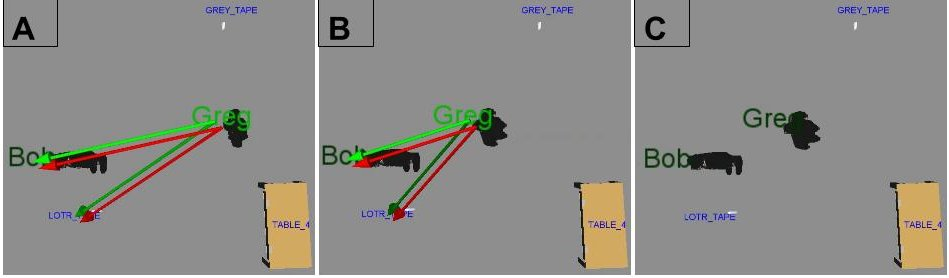
\includegraphics[width=0.90\textwidth]{img/movingToward.jpg}
 \end{tabular}
 \caption{Representation of the facts IsMoving and IsMovingToward.}
 \label{fig:mvTwd}
 \end{figure}

When the monitored agent is not moving, we compute some facts concerning its monitored joints.
We compute in a similar manner the facts \textit{IsMoving} and \textit{IsMovingToward} so we won't detail it again.
We also compute facts concerning distances between the monitored joint and other entities:

 \textbf{Distance}: this fact is computed only if the agent is not moving.
To compute this, we basically compute the 3d distance between the joint monitored and the other entities of the environment.

The \textit{property} is \textit{Distance}, the \textit{propertyType} is \textit{position}, the \textit{subProperty} is set with \textit{3D}, the \textit{subjectId} is the id of the monitored agent's joint, \textit{subjectOwnerId} is set with the id of the monitored agent. The \textit{targetId} is the id of the entity we compute the distance with. The \textit{time} is set with the perception time of the monitored agent, the \textit{valueType} is set to zero, the \textit{stringValue} is set to \textit{"reach", "close", "medium", "far"} or \textit{"out"} according to the distance value. These threshold can be changed using ros dynamic reconfigure. The \textit{doubleValue} is set with the actual distance value between the agent joint's and the entity.

\textbf{example:} \textit{RIGHT\_HAND BOB Distance BLUE\_BOOK reach  ...}


\textbf{Note:} To get reliable data for \textit{isMovingToward}, you may want to combine both facts (direction and distance).
 
\subsection{Inputs}
This component of TOASTER reads the topics published by PDG and uses it as inputs to compute required facts.

\subsection{Outputs}
It publishes facts like IsMoving, IsMovingToward, IsLookingToward, Distance on topic /agent\_monitor/factList.

\subsection{Services}
Main services of agent\_monitor are :

\begin{itemize}
\item \textbf{add\_agent} - This service adds agent to the list of agents to be monitored by this module. It takes string id of the agent to be added. Similarly, add\_joint\_to\_agent service adds joint of an agent to the list of joints to be monitored closely by the agent\_monitor.

\textbf{Shell command:}

\textit{rosservice call /agent\_monitor/add\_agent "id: ''" }

\item \textbf {remove\_agent} - This service removes agent from the list of agents to be monitored by this module. It takes string id of the agent to be removed. Similarly, working of other services like remove\_all\_agents, remove\_all\_joints\_to\_agent, remove\_joint\_to\_agent, monitor\_all\_agents can be understood by their names.

\item \textbf{pointing} - It gives the id of the entity towards which the given joint of an agent is pointing with some level of confidence. It is computed for given threshold of pointing distance and angle threshold.


\textbf{Shell command:}

\textit{rosservice call /agent\_monitor/pointing "pointingAgentId: 'HERAKLES\_HUMAN1'
pointingJoint: ''
pointingJointDistThreshold: 0.0
angleThreshold: 0.0"}

Similarly, the service pointing\_time shows the id of agent towards which given joint of an agent is pointing at a given pointing time.

\end{itemize}

\subsection{Examples}
Using the circular buffer we are able to know what the human was pointing at, at a given moment. This can be useful for a fusion component of a dialog system. As an example, if a human asks "give me that", if the speech recognition is able to provide the time when the human said "that", we can request to the agent monitor component what objects were pointed by the human at this time.
This fact is computed on request. The request returns a list of entities with a probability on each candidates.

\subsection{Future work and possible improvement}
The computation in agent\_monitor are basically using the data of the agent or entity at a previous time and we compare it with the last data. A better way to compute facts concerning motion would be to use more than two point of time and using filters like Kalman or better way to use the circular buffer to avoid windowing effect.

As mentioned before, we could also have conditional computation to minimize the resource consumption.




%%%%%%%%%%%%%%%%%%%%%%%%%%%%%%%%%%%%%%
\section{move3d\_facts}
\textbf{NOTE:} This is currently a work in progress.

One of the components is responsible for the spatial relation computation. It makes a 3d representation of the world state and computes properties to describe relations between objects (such as \textit{isIn}, \textit{isOn}, \textit{isNextTo}) and affordances of agents toward objects (\textit{canSee}, \textit{canReach}). One can make requests concerning the relative position of entities toward an agent's point of view. This kind of requests enhance the robot with a geometrical perspective taking ability to talk to the human with his own references, improving the social aspect of the system.


\subsection{Facts computation}
%TODO: list of computed facts and how are they computed?

The fact list will be given once the module integrated to the toaster architecture.


\subsection{Inputs}
This module subscribes to topics /agent\_monitor/factList and /area\_manager/factList.
\subsection{Outputs}
It does computation in 3-dimensions and publishes facts like isVisible, isReachableBy, isOn, isIn on /move3d\_facts/factLsit topic.
\subsection{Services}
This component has no services.
\subsection{Examples}
 As an example the facts (simplified here) <\textit{BLUE\_BOOK isIn BOX1}> or <\textit{HUMAN1 canReach BOX1}> can be generated by this module.It can also tell the relative position of an entity, compared to another, from the agent's perspective. For example, it makes possible for the robot to tell to the human "the mug you are looking for is \textbf{on your right}" or "please give me the book which is \textbf{for you on the left of the red mug}".
\subsection{Future work and possible improvement}

%%%%%%%%%%%%%%%%%%%%%%%%%%%%%%%%%%%%%%
\section{belief\_manager}
This component is an older version of \textit{database\_manager} module of TOASTER. It updates the world states on observing the changes in agent's surrounding. It enhances the robotic system with Theory of Mind skills and more specifically conceptual perspective taking. To do so, it maintains a belief state for the robot, which comes from the world state, and assesses the belief state of the other agents.
In the latest version of TOASTER, this functionality has been embedded into database\_manager node.


\subsection{Implementation details}
A belief state is a symbolic representation of a world state, i.e. a set of facts that the agent believes to be true at a given time. Agents can have a different representation of the world, resulting in different Belief states.A belief state is a symbolic representation of a world state, i.e. a set of facts that the agent believes to be true at a given time. Agents can have a different representation of the world, resulting in different Belief states.We implemented a rule based fact reasoning process in order to build belief state of each agent and update it when needed. Human belief models are updated using the awareness on the human perception affordances. When the robot's belief model is updated, the robot checks that the humans are able to perceive the changes in the environment before updating their belief state. To be aware of the changes in the environment a human needs either to observe the \textit{event} (there is an \textit{event} when a change in the environment occurs, such as an action performed by an agent), or to directly observe the new world state and the changes produced in the. The management of the former case of update is made by the supervision layer which assesses if the human is able to perceive the event. This decision can rely, (1) on the fact that the human is in the same room, and (2) on the visual affordances of the human toward entities implied in the event.
For the later case of update, we use the human visibility toward the subject of the property, combined with the observability of the given property, to assess if the human is able to update his belief on the world state. The confidence on the fact that the human is aware of the new property is computed by combining the confidence on the human visibility toward the subject of the current fact to update and the observability of the fact itself.
This way, if an object is hard to perceive by the human (partially occluded), or if the property is hard to observe (low observability), the robot will have a low confidence on the fact that the human actually holds this belief.

\subsection{Examples}
As an example, if a human \textit{H} is not aware that a cup has been filled with hot water, and if he can't see properly the cup, the property \textit{hotCup} will have a low confidence in \textit{H} belief's state.
An other example, if the human \textit{H} is away when an agent \textit{A} fills the cookie-box, when \textit{H} comes back, if the cookie-box is closed, the fact that it is filled won't be observable (observability null). Consequently, \textit{H} mental state will still have the fact \textit{cookie-box isEmpty} set at \textit{TRUE} in his belief state (resulting in a false belief situation).


%%%%%%%%%%%%%%%%%%%%%%%%%%%%%%%%%%%%%%
\section{database\_manager}
To store and manage the facts generated from Spatial and Temporal Reasoning components, and to add a memory to our system, we created a module based on a SQL Temporal Database. Apart from the conceptual perspective taking (as described in belief\_manager), another capacity of the database component is the event based time management. This provides memory to the system.
When facts are received, the time of detection is present in one of their variables. When the database manager detects a shift in a property, it updates the belief tables as explained in previous section, but it also records the event. To do so, we add a table filled with each event that occurs, recording the time when the property changes. This is a significant component of TOASTER as it is used for testing and debugging this situation assessment framework.


\subsection{Implementation details}
This module continuously reads facts from PDG, area\_manager, agent\_monitor and move3d\_facts. All these facts are updated in the robot's belief state. Once the robot belief state is updated, it updates the other agent's belief state by the idea of conceptual perspective taking. Refer to Fig.~\ref{fig:databaseManager} for better understanding.
 \begin{figure}[ht!]
 \centering
 \begin{tabular}{cc}
  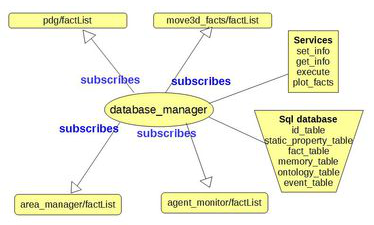
\includegraphics[width=0.90\textwidth]{img/database.png}
 \end{tabular}
 \caption{Implementation of database\_manager module}
 \label{fig:databaseManager}
 \end{figure}

\subsection{Inputs}
To maintain robot's own belief state, the information produced by perception, geometrical reasoning and inferences are collected by the database management module. Facts computed from area\_manger, agent\_monitor and move3d\_facts are stored in this module. 
\subsection{Outputs}
The output of this component is a sql database with fact table and memory table for each agent present in ID table. The fact table stores all the fact true for the agent at that time instant. While, the memory table stores facts that the agent has believed to be true. There is an event table as well to track the occurrence of events like when robot started moving and when it stopped moving. However, during an interaction, many properties that describes an object or an agent may not evolve in time and thus, be considered as static (color, name, age, ownership). To store these static properties, an extra table is present in the database and can be loaded at the start of the interaction, or filled online (if the robot acquire new knowledge on entities). For more details, check \url{https://github.com/Greg8978/toaster/blob/master/database\_manager/doc/database\%20doc.pdf}.

\subsection{Services}
Services of database\_manager allows you to add entity, facts and events in respective tables and view all the tables. Its services are described below :
\begin{itemize}
\item \textbf {execute} - This service enables users to access the data in tables in various ways by putting different commands.

\textbf{Shell command:}

\textit{rosservice call /database/execute "command: ''
type: ''
facts:
- {property: '', propertyType: '', subProperty: '', subjectId: '', targetId: '', subjectOwnerId: '',
  targetOwnerId: '', valueType: false, factObservability: 0.0, doubleValue: 0.0, stringValue: '',
  confidence: 0.0, time: 0, timeStart: 0, timeEnd: 0}
agent: ''
order: ''
areaTopic: false
agentTopic: false
move3dTopic: false
pdgTopic: false" 
}

Set the \textit{areaTopic, agentTopic, move3dTopic, pdgTopic} as per your requirement. Using command "ARE\_IN\_TABLE" with agent and facts, it checks if the given facts are present in agent's fact table. "SQL" command with the query in order request message, executes the SQL query in database and displays the results. The command "EMPTY" with type "AGENT" for a given agent removed that agent from ID table and other tables related to this agent. With "ALL" type, it does the same for all agents. Using command "PRINT" with type "AGENT" prints tables of the given agent, while type "ALL" prints all tables in database.

\item \textbf {get\_info} - This service helps to get data from any given table. With the combination of type as "FACT" and subType as "ALL", it displays all the facts in the given agent's table at current time and before that also. While subType "VALUE", shows value of the given fact for the specified agent at current time. The subType "CURRENT" gives all the current facts of the given agent while "OLD" displays older facts. Similarly, combination of "ALL" subType with type as "EVENT", "ONTOLOGY", "ID" and "PROPERTY" displays respective tables from database. While subtype "VALUE" with all possible type gives values from respective tables. The request message looks like this :

\textbf{Shell command:}

rosservice call /database/get\_info "type: ''
subType: ''
agentId: ''
reqFact: {property: '', propertyType: '', subProperty: '', subjectId: '', targetId: '',
  subjectOwnerId: '', targetOwnerId: '', valueType: false, factObservability: 0.0,
  doubleValue: 0.0, stringValue: '', confidence: 0.0, time: 0, timeStart: 0, timeEnd: 0}
reqEvent: {property: '', propertyType: '', subProperty: '', subjectId: '', targetId: '',
  subjectOwnerId: '', targetOwnerId: '', valueType: false, factObservability: 0.0,
  doubleValue: 0.0, stringValue: '', confidence: 0.0, time: 0}
id: 0
idString: ''
name: ''
entityClass: ''" 

\item \textbf {plot\_facts} - This service is developed with the purpose of examining the functioning of TOASTER in real-time environment. It plots the given fact for the given subject and target entity in specified time window. This service creates "fact.dat" file in your home directory. To plot the graph install gnuplot and run "gnuplot" command on terminal. In gnuplot terminal, run following commands:

\textit{gnuplot> set yrange[-1:2]}

\textit{gnuplot>  plot "fact.dat" using 1:2 with lines}
And you will see the desired plot. 

\textbf{Shell command:}

rosservice call /database/plot\_facts "{subjectID: '', targetID: '', timeStart: '', timeEnd: '', reqFact: ''}"

\item \textbf {set\_info} - 

\textbf{Shell command:}

\textit{rosservice call /database/set\_info "add: false
infoType: ''
agentId: ''
facts:
- {property: '', propertyType: '', subProperty: '', subjectId: '', targetId: '', subjectOwnerId: '',
  targetOwnerId: '', valueType: false, factObservability: 0.0, doubleValue: 0.0, stringValue: '',
  confidence: 0.0, time: 0, timeStart: 0, timeEnd: 0}
event: {property: '', propertyType: '', subProperty: '', subjectId: '', targetId: '',
  subjectOwnerId: '', targetOwnerId: '', valueType: false, factObservability: 0.0,
  doubleValue: 0.0, stringValue: '', confidence: 0.0, time: 0}
id: ''
name: ''
type: ''
ownerId: ''"} 
\end{itemize}
\subsection{Examples}
 As an example, if a Mug was on a table and the robot detects that the Mug is now in Bob's hand, it will remove the fact $<$\textit{Mug isOn $Kithen\_Table$}$>$ from the belief tables of agents able to perceive the change, and add the event $<$\textit{Bob pickUp Mug}$>$ in the event table.
In memory table, we use as starting time the time when the agent noticed a property, and as ending time the moment when the agent detects a change in it.
One of the application can be to understand when a human asks "Where is the mug that was on the table" by detecting in his memory table which mug she/he is talking about and looking in the current fact table where it currently is. In addition, the robot could even tell the related event that created the change: "It is now in the sink, Bob picked it up 5 minutes ago".

\subsection{Future work and possible improvement}
This module is one of the last implementation of TOASTER. More tests should be done to ensure the database is able to answer fast enough to the requests.



%%%%%%%%%%%%%%%%%%%%%%%%%%%%%%%%%%%%%%
\section{toaster\_visualizer}
To understand the situation and visualize the internal processes, a visualization module is rendering the names and 3d models at the position of the entities and the areas with their names, 
\footnote{http://wiki.ros.org/rviz}.
This visualization simplifies the debugging process and allows a faster setup of the framework parameters. This module is designed to create a simple 3d representation of toaster's physical elements in RVIZ.

\subsection{Implementation details}
Fig.~\ref{fig:visualizer}  explains the implementation of this module. To use rviz with TOASTER, follow the configuration instructions at \url{https://github.com/Greg8978/toaster/blob/master/toaster_visualizer/doc/toaster_visualizer_doc.pdf}
 \begin{figure}[ht!]

 \centering
 \begin{tabular}{cc}
  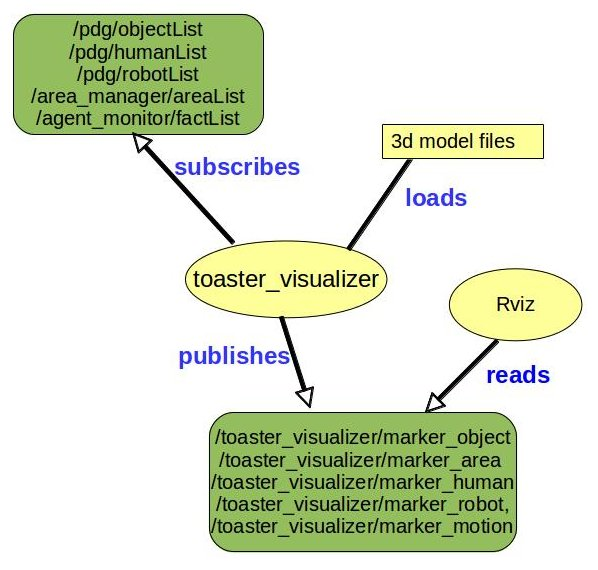
\includegraphics[width=0.9\textwidth]{img/visualizer.jpg}
 \end{tabular}
 \caption{Implementation of toaster\_visualizer module}
 \label{fig:visualizer}
 \end{figure}
\subsection{Inputs}
It uses the position of the entities published by the data gathering component and the areas published by the area manager component Toaster\_visualizer use informations taken form toaster\_msgs published on specifics ros topics to create markerArray.
toaster\_msgs concerned: AreaList, ObjectList, HumanList
topics concerned: /area\_manager/areaList, /pdg/objList, /pdg/humanList

\subsection{Outputs}
It publishes markerArray on topics like /toaster\_visualizer/marker\_area, marker\_human, marker\_robot, marker\_motion and marker\_objects viewable with RVIZ as shown in Fig.~\ref{fig:simu} and Fig.~\ref{fig:spencer}. For more details, you can check https://github.com/Greg8978/toaster/blob/master/toaster\_visualizer/doc/toaster\_visualizer\_doc.pdf.
 \begin{figure}[ht!]

 \centering
 \begin{tabular}{cc}
  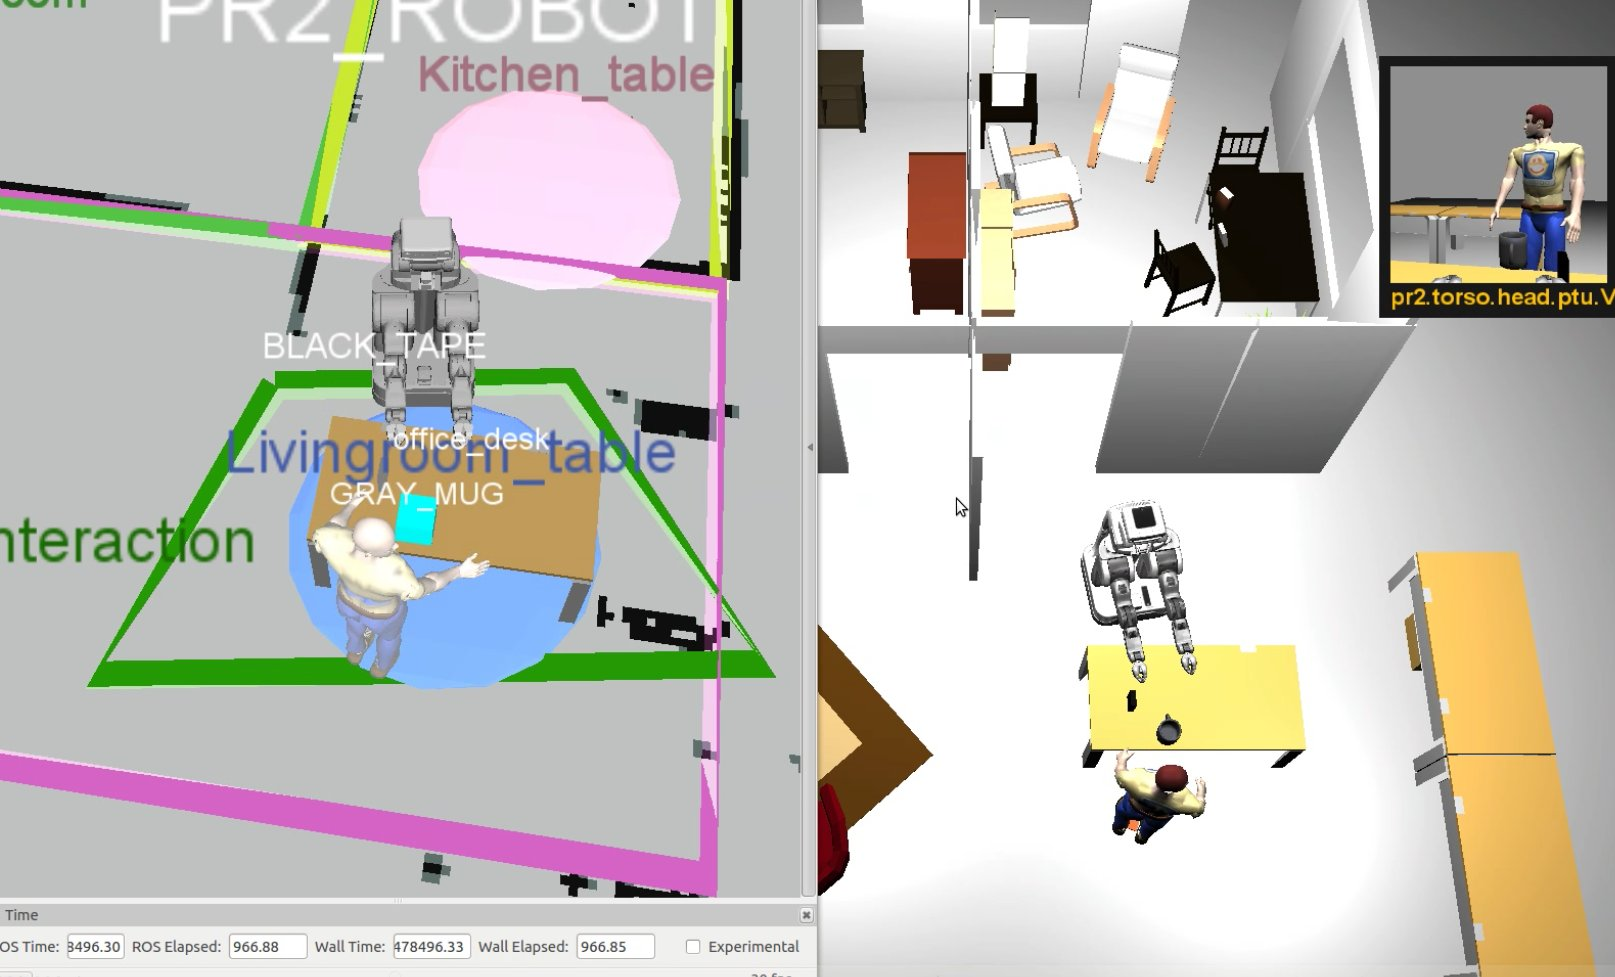
\includegraphics[width=0.9\textwidth]{img/tosaster.jpg}
 \end{tabular}
 \caption{Data from simulated sensors in MORSE (right) and its representation in TOASTER (left)}
 \label{fig:simu}
 \end{figure}
 
 \begin{figure}[ht!]
 \centering
 \begin{tabular}{cc}
  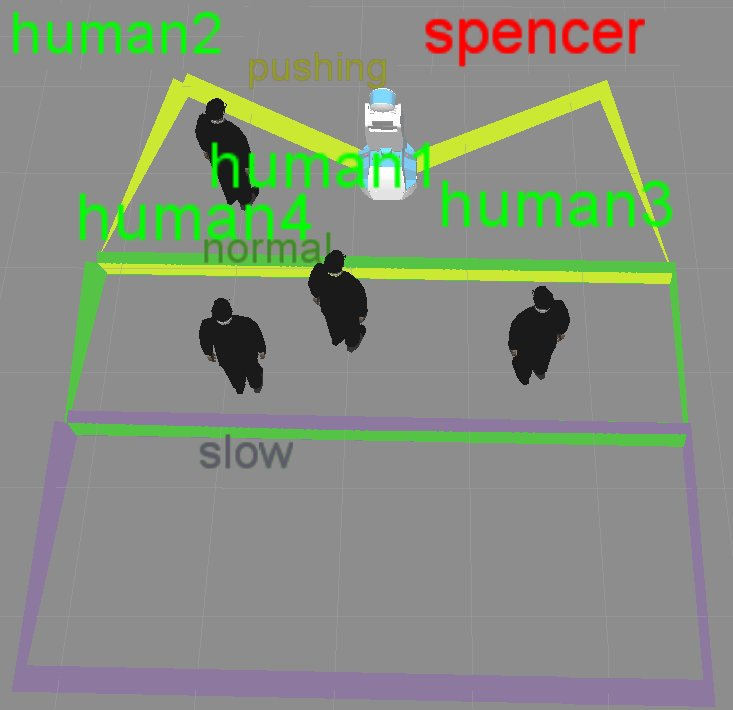
\includegraphics[width=0.45\textwidth]{img/toaster_spencer.jpg} &
  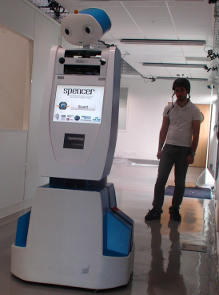
\includegraphics[width=0.4\textwidth]{img/spencer_guidingShrink.png}
 \end{tabular}
 \caption{Spencer robot and its attached areas for guiding humans, in TOASTER (left) and in the real world (right)}
 \label{fig:spencer}
 \end{figure}
\subsection{Services}
This node has no services.

\subsection{Future work and possible improvement}
In a future work, we would like to improve this visualization by adding the rendering of other facts, such as the one generated by the agent monitoring component about the attention.


\section{Facts computation recapitulation}

To help understanding and to give a global view of the facts computation, we give in the following table the recapitulation of all the facts computed in TOASTER along with the module computing it.

%TODO add ref to explanation in this doc

\begin{sidewaystable}
 %\vspace{-10pt}
\centering
\renewcommand{\arraystretch}{1.0}
\begin{tabular}{|c|c|c|c|c|c|c|c|c|}
\hline


\textbf{node} & Property & PropType & Subproperty & subjectId & TargetId & stringValue & doubleValue & brief description \\
\hline
\hline

\textbf{PDG} & IsSeen & affordance & $\emptyset$ & \textit{obj.id} & $\emptyset$ & true & $\emptyset$ & Object is perceived from sensor(s)  \\
\hline


\textbf{PDG} & IsInHand & position & object & \textit{obj.id} & \textit{joint.id} & true & $\emptyset$ & From pdg service put\_in\_hand  \\
\hline
\hline

\textbf{area\_man} & IsInRoom & position & room & \textit{ent.id} & \textit{area.name} & true & $\emptyset$ & If subject is inside room area  \\
\hline

\textbf{area\_man} & IsAt & position & location & \textit{ent.id} & \textit{area.name} & true & $\emptyset$ & If subject is inside support area  \\
\hline

\textbf{area\_man} & IsInArea & position & location & \textit{ent.id} & \textit{area.name} & true & $\emptyset$ & If subject is inside other area  \\
\hline


\textbf{area\_man} & AreaDensity & density & ratio & \textit{area.name} & $\emptyset$ & $\emptyset$ & \textit{EntArea}/\textit{Ent} & compute if area.factType=density  \\
\hline

\textbf{area\_man} & IsFacing & posture & angle & \textit{ent.id} & \textit{ent.id} & true & \textit{angle} & compute if area.factType=interaction  \\
\hline
\hline

\textbf{agt\_mon} & IsLookingTwd & attention & agent & \textit{agt.id} & \textit{ent.id} & true& $\emptyset$ & angle cone from agent's head  \\
\hline

\textbf{agt\_mon} & IsMoving & motion & agent & \textit{agt.id} & $\emptyset$ & true & $\emptyset$ & \textit{speed} $>$ 0.12 m/s  \\
\hline

\textbf{agt\_mon} & IsMoving & motion & joint & \textit{jnt.name} & $\emptyset$ & true & $\emptyset$ & \textit{speed} $>$ 0.12 m/s \\
\hline

\textbf{agt\_mon} & IsMovingTwd & motion & direction & \textit{agt.id} & \textit{ent.id} & true & \textit{angle} & trajectory of agent is toward ent  \\
\hline

\textbf{agt\_mon} & IsMovingTwd & motion & direction & \textit{jnt.name} & \textit{ent.id} & true & \textit{angle} & trajectory of \textit{jnt} is toward \textit{ent}  \\
\hline

\textbf{agt\_mon} & IsMovingTwd & motion & distance & \textit{agt.id} & \textit{ent.id} & true & \textit{dist} & distance agt/ent decreasing  \\
\hline

\textbf{agt\_mon} & IsMovingTwd & motion & distance & \textit{jnt.name} & \textit{ent.id} & true & \textit{dist} & \textit{dist} \textit{jnt}/{ent} decreasing  \\
\hline

\textbf{agt\_mon} & Distance & position & 3D & \textit{jnt.name} & \textit{ent.id} & \textit{distStr} & \textit{dist} & distance \textit{jnt}/ent decreasing  \\
\hline




\end{tabular}
\caption{Facts computed by TOASTER framework}
%    \vspace{-10pt}
 \label{table:facts}


\end{sidewaystable}

\clearpage

\bibliographystyle{IEEEtran}
\bibliography{intention,situation_assessment}


\end{document}
